\documentclass{article}
\usepackage{xeCJK} 
\usepackage{amsmath}
\usepackage{amsfonts}
\usepackage{amssymb}
\usepackage{graphicx} 
\usepackage{tikz}


\setCJKmainfont{SimSun}
\usetikzlibrary{shapes.geometric, arrows}

\tikzstyle{startstop} = [rectangle, rounded corners, minimum width=3cm, minimum height=1cm, text centered, draw=black, fill=red!30]
\tikzstyle{process} = [rectangle, minimum width=3cm, minimum height=1cm, text centered, draw=black, fill=blue!20]
\tikzstyle{decision} = [diamond, minimum width=3.5cm, minimum height=1cm, text centered, draw=black, fill=green!20]
\tikzstyle{arrow} = [thick,->,>=stealth]

\begin{document}
\title{PRML第二次作业}
\author{许书闻 2023K8009926005}
\maketitle

\section*{第1题}
(1)

(i)Fisher判别准则:
最小化类内散度矩阵,最大化类间散度矩阵,
从而得到一个最优的投影方向,使得投影后的数据在该方向上的方差最大,
不同类别的数据在该方向上的均值尽可能远离,从而实现分类的目的。

优化目标:
找到一个投影方向作为分类超平面的法向,最小化类内散度矩阵,最大化类间散度矩阵。

求解过程如下:

step1. 类内散度矩阵 \( S_W \),
对于每一类 \( C_k \),类内散度矩阵定义为:
\[
S_W = \sum_{k=1}^{K} \sum_{\mathbf{x}_i \in C_k} (\mathbf{x}_i - \mu_k)(\mathbf{x}_i - \mu_k)^T
\]
其中,\( \mu_k \) 是类别 \( C_k \) 的均值向量,定义为:
\[
\mu_k = \frac{1}{N_k} \sum_{\mathbf{x}_i \in C_k} \mathbf{x}_i
\]

step2. 类间散度矩阵 \( S_B \),
类间散度矩阵度量了不同类别样本之间的散布程度。类间散度矩阵定义为:
\[
S_B = \sum_{k=1}^{K} N_k (\mu_k - \mu)(\mu_k - \mu)^T
\]

其中,\( N_k \) 是类别 \( C_k \) 中样本的数量,\( \mu_k \) 是类别 \( C_k \) 的均值向量,\( \mu \) 是所有样本的全局均值向量,定义为:

\[
\mu = \frac{1}{N} \sum_{i=1}^{N} \mathbf{x}_i
\]

其中,\( N \) 是总样本数。

step3. 优化目标
目标函数 \( J(\mathbf{w}) \) 定义为:
\[
J(\mathbf{w}) = \frac{\mathbf{w}^T S_B \mathbf{w}}{\mathbf{w}^T S_W \mathbf{w}}
\]
要选择一个投影方向 \( \mathbf{w} \),使得目标函数 \( J(\mathbf{w}) \) 最大化。

这是一个广义瑞利商问题,可以用拉格朗日乘子法求解。为简化问题,可以标准化地设\(\mathbf{w}^T \mathbf{S_B}\mathbf{w} = 1\)。

构造拉格朗日函数:

\[
\mathcal{L}(\mathbf{w}, \lambda) = \mathbf{w}^T S_B \mathbf{w} - \lambda (\mathbf{w}^T S_W \mathbf{w} - 1)
\]

对 \( \mathbf{w} \) 和 \( \lambda \) 求偏导,并令其为零:

得到方程:

\[
(S_B - \lambda S_W) \mathbf{w} = 0
\]

\[
\mathbf{w}^T S_W \mathbf{w} = 1
\]
这表明,\( \mathbf{w} \) 是矩阵 \( S_W^{-1} S_B \) 的特征向量。

step4. 求解特征值问题
\[
S_W^{-1} S_B \mathbf{w} = \lambda \mathbf{w}
\]得到的解$\mathbf{w}$即为最优的投影方向。

根据一维投影值 \( y \) 来进行分类。通常,如果样本投影值大于某个阈值,则预测为一类,否则预测为另一类。

(ii)感知机:
感知机是一种线性分类模型,属于判别模型。
感知机模型的假设空间是定义在特征空间中的所有线性分类模型或线性分类器,
线性判别函数是 \( g(\mathbf{z}) = \alpha^T z\)。\\
其中增广样本向量$z=[1,x_1,x_2,...,x_d]^T$,权向量$\alpha=[\alpha_0,\alpha_1,\alpha_2,...,\alpha_d]^T$。

目标:找到一个超平面,使得正负样本能够被分开。(在样本线性可分时保证具有收敛性)

求解过程如下,定义感知机准则函数:
\[J_p(\alpha)=\sum_{\alpha^T z_k t_k}(-\alpha^Tz_k t_k)\]

step1. 选择一个初始权向量 \( \alpha \)。通常可以随机,并置$t=0$。

step2.对于每一个样本$z_j$,若$\alpha(t)^Tz_t t_k\leq0,$则$\alpha(t+1)=\alpha(t)+z_kt_k$,否则继续。

step3.考察另一个样本,重复步骤2,直至对所有样本都有$\alpha(t)^Tz_t t_k>0$,即$J_p(\alpha)=0$。

(iii)Logistic回归:

优化目标:通过一个线性模型预测事件发生的概率。
其输出是一个概率值,通常使用Sigmoid函数来描述。

求解过程如下:
step1. 假设函数:

在Logistic回归中,我们假设类别为1的概率是由以下模型给出的:

\[
P(y = 1 | \mathbf{x}) = \sigma(\mathbf{w}^T \mathbf{x}) = \frac{1}{1 + e^{-\mathbf{w}^T \mathbf{x}}}
\]

其中,\( \sigma(z) \) 是Sigmoid函数,定义为:

\[
\sigma(z) = \frac{1}{1 + e^{-z}}
\]

\(\mathbf{w}^T \mathbf{x}\) 是线性模型的输出,表示输入特征的加权和。

step2. 目标函数 (对数似然函数)

Logistic回归的目标是找到参数 \( \mathbf{w} \),使得预测概率与实际标签之间的差异最小。我们采用对数似然函数来衡量模型的拟合度。

对于一个训练集 \( \{(\mathbf{x}_i, y_i)\}_{i=1}^{N} \),其中 \( \mathbf{x}_i \) 是第 \(i\) 个样本,\( y_i \in \{0, 1\} \) 是对应的标签。对数似然函数 \( \ell(\mathbf{w}) \) 定义为:

\[
\ell(\mathbf{w}) = \sum_{i=1}^{N} \left[ y_i \log(\sigma(\mathbf{w}^T \mathbf{x}_i)) + (1 - y_i) \log(1 - \sigma(\mathbf{w}^T \mathbf{x}_i)) \right]
\]

优化目标 (最大化对数似然函数) 等价于最小化负对数似然函数(又称为二值交叉熵) \( L(\mathbf{w}) \):

\[
L(\mathbf{w}) = - \ell(\mathbf{w}) = - \sum_{i=1}^{N} \left[ y_i \log(\sigma(\mathbf{w}^T \mathbf{x}_i)) + (1 - y_i) \log(1 - \sigma(\mathbf{w}^T \mathbf{x}_i)) \right]
\]

step3. 求梯度:

我们对 \( L(\mathbf{w}) \) 关于 \( \mathbf{w} \) 求导,并通过链式法则进行化简。

先对 \( y_i \log(\sigma(\mathbf{w}^T \mathbf{x}_i)) \) 求导:

\[
\frac{\partial}{\partial \mathbf{w}} \left[ y_i \log(\sigma(\mathbf{w}^T \mathbf{x}_i)) \right]
\]

应用链式法则,得到:

\[
\frac{\partial}{\partial \mathbf{w}} \log(\sigma(\mathbf{w}^T \mathbf{x}_i)) = \frac{1}{\sigma(\mathbf{w}^T \mathbf{x}_i)} \cdot \frac{\partial}{\partial \mathbf{w}} \sigma(\mathbf{w}^T \mathbf{x}_i)
\]

因为sigmoid函数满足: \( \frac{d}{dz} \sigma(z) = \sigma(z)(1 - \sigma(z)) \),所以:

\[
\frac{\partial}{\partial \mathbf{w}} \sigma(\mathbf{w}^T \mathbf{x}_i) = \sigma(\mathbf{w}^T \mathbf{x}_i) \left( 1 - \sigma(\mathbf{w}^T \mathbf{x}_i) \right) \mathbf{x}_i
\]

因此,

\[
\frac{\partial}{\partial \mathbf{w}} \left[ y_i \log(\sigma(\mathbf{w}^T \mathbf{x}_i)) \right] = y_i \left( 1 - \sigma(\mathbf{w}^T \mathbf{x}_i) \right) \mathbf{x}_i
\]

再对 \( (1 - y_i) \log(1 - \sigma(\mathbf{w}^T \mathbf{x}_i)) \) 求导:

\[
\frac{\partial}{\partial \mathbf{w}} \left[ (1 - y_i) \log(1 - \sigma(\mathbf{w}^T \mathbf{x}_i)) \right]
\]

同样应用链式法则,得到:

\[
\frac{\partial}{\partial \mathbf{w}} \log(1 - \sigma(\mathbf{w}^T \mathbf{x}_i)) = \frac{-1}{1 - \sigma(\mathbf{w}^T \mathbf{x}_i)} \cdot \frac{\partial}{\partial \mathbf{w}} \sigma(\mathbf{w}^T \mathbf{x}_i)
\]

所以:

\[
\frac{\partial}{\partial \mathbf{w}} \sigma(\mathbf{w}^T \mathbf{x}_i) = \sigma(\mathbf{w}^T \mathbf{x}_i) \left( 1 - \sigma(\mathbf{w}^T \mathbf{x}_i) \right) \mathbf{x}_i
\]

因此,

\[
\frac{\partial}{\partial \mathbf{w}} \left[ (1 - y_i) \log(1 - \sigma(\mathbf{w}^T \mathbf{x}_i)) \right] = -(1 - y_i) \sigma(\mathbf{w}^T \mathbf{x}_i) \mathbf{x}_i
\]

合并两项结果,得到梯度:

\[
\frac{\partial L(\mathbf{w})}{\partial \mathbf{w}} = - \sum_{i=1}^{N} \left[ y_i \left( 1 - \sigma(\mathbf{w}^T \mathbf{x}_i) \right) \mathbf{x}_i - (1 - y_i) \sigma(\mathbf{w}^T \mathbf{x}_i) \mathbf{x}_i \right]
\]

我们将项合并,得到最终简化的结果:
\[
\frac{\partial L(\mathbf{w})}{\partial \mathbf{w}} = \sum_{i=1}^{N} \left[ \sigma(\mathbf{w}^T \mathbf{x}_i) - y_i \right] \mathbf{x}_i
\]
step4.使用梯度下降法更新参数 \( \mathbf{w} \):
\[
\mathbf{w} \leftarrow \mathbf{w} - \eta \frac{\partial L(\mathbf{w})}{\partial \mathbf{w}}
\]
其中,\( \eta \) 是学习率,控制每次更新的步长。

step5. 结果与分类:

训练完成后,使用得到的 \( \mathbf{w} \) 来进行预测。对于一个新的样本 \( \mathbf{x} \),我们计算:
\[
P(y = 1 | \mathbf{x}) = \sigma(\mathbf{w}^T \mathbf{x})
\]
根据预测的概率 \( P(y = 1 | \mathbf{x}) \),如果大于 0.5,则预测为类别 1;否则,预测为类别 0。

(2)最小二乘法求解步骤:

step1. 定义损失函数

最小二乘法的目标是最小化预测值与实际值之间的误差。
假设模型为 \( y = \mathbf{w}^T \mathbf{x} \),其中$w=[w_0,w_1,...,w_d]^T$是待定参数,$x=[1,x_1,...,x_N]^T$是增广样本向量。则误差的平方和(损失函数)为:
\[
L(\mathbf{w}) = \sum_{i=1}^{N} \left( y_i - \mathbf{w}^T \mathbf{x}_i  \right)^2
\]
step2. 对$w$求导数,得到损失函数的最小值及其条件

写成矩阵形式,即:

$$L(w)=\frac{1}{N}\sum_{i=1}^{N}(\mathbf{w}^T\mathbf{x}_i-y_i)^2=\frac{1}{N}(\mathbf{Xw}-\mathbf{y})^T(\mathbf{Xw}-\mathbf{y})$$

其中$X$是增广样本矩阵,$y$是标签向量。

对$w$求导,得到:
$$\frac{\partial L(w)}{\partial w}=\frac{2}{N}\mathbf{X}^T(\mathbf{Xw}-\mathbf{y})=0$$
即:$$\mathbf{X}^T\mathbf{Xw}=\mathbf{X}^T\mathbf{y}$$

最小二乘法具有解析解的条件是:矩阵 \( \mathbf{X}^T \mathbf{X} \) 必须是可逆的,即要求矩阵 \( \mathbf{X}^T \mathbf{X} \) 是非奇异的。

当矩阵 \( \mathbf{X}^T \mathbf{X} \) 是非奇异的时候,最小二乘法的解析解为:
$$\mathbf{w} = (\mathbf{X}^T \mathbf{X})^{-1} \mathbf{X}^T \mathbf{y}$$

(3)梯度下降法和随机梯度下降法的区别:

在每次迭代中,计算所有样本的梯度(即损失函数关于模型参数的偏导数)的方法称为梯度下降法(GD);

而随机梯度下降法(SGD)在每次迭代中只使用一个样本的梯度来更新模型参数。


优缺点对比:
梯度下降法(GD)

a.优点:

全局最优解:由于每次迭代都使用所有数据,梯度的计算比较精确,因此梯度下降法在凸优化问题中可以保证收敛到全局最优解。

收敛稳定:梯度下降法的更新步骤较为平稳,通常在收敛时非常稳定。

b.缺点:

计算开销大:每次迭代都需要对所有训练样本进行梯度计算,对于大规模数据集,计算开销非常大,训练时间长。

速度较慢:每次迭代都涉及对所有数据进行梯度计算,因此每次迭代的更新比较慢,收敛速度较慢。

随机梯度下降法(SGD)的优缺点
a.优点:

计算效率高:每次更新只使用一个样本,计算量大大减少,适用于大规模数据集,训练速度较快。

收敛速度快:由于每次迭代使用的数据量小,更新频繁,因此收敛速度较快(但有时收敛到的解可能是一个局部最优解,尤其在非凸问题中)。

适应性强:适合在线学习,可以随时加入新的数据。

b.缺点:

收敛不稳定:由于每次更新只有一个样本,梯度方向可能有很大的波动,导致收敛过程不稳定,甚至可能永远无法精确收敛到最优解。

局部最优解:在非凸优化问题中,SGD有可能陷入局部最优解。

\section*{第2题}
(1)最优分类超平面是指一个分类超平面,能将训练样本没有错误地分开,
且两类训练样本中离超平面最近的样本与超平面之间的距离是最大的。\\
支持向量机(SVM)通过求解最优分类超平面来实现数据的最大间隔分类。\\
(2)支持向量是指离分类超平面最近的样本点,这些样本点到分类超平面的距离是最小的。

(i)原问题(Primal Problem) \\
给定训练数据集:
\[
\{(\mathbf{x}_i, y_i) \}_{i=1}^{N}, \quad y_i \in \{-1, 1\}, \quad \mathbf{x}_i \in \mathbb{R}^d
\]
SVM 目标是找到最优分类超平面:
\[
\mathbf{w}^T \mathbf{x} + b = 0
\]
以最大化间隔,同时满足约束条件:
\[
y_i (\mathbf{w}^T \mathbf{x}_i + b) \geq 1, \quad \forall i = 1, 2, \dots, N
\]
从而优化问题可表示为:
\[
\min_{\mathbf{w}, b} \quad \frac{1}{2} \|\mathbf{w}\|^2
\]
\[
\text{s.t.} \quad y_i (\mathbf{w}^T \mathbf{x}_i + b) \geq 1, \quad \forall i
\]
拉格朗日函数构造:\\
引入拉格朗日乘子 \( \alpha_i \geq 0 \),构造拉格朗日函数:
\[
L(\mathbf{w}, b, \boldsymbol{\alpha}) = \frac{1}{2} \|\mathbf{w}\|^2 - \sum_{i=1}^{N} \alpha_i [y_i (\mathbf{w}^T \mathbf{x}_i + b) - 1]
\]
对 \( \mathbf{w} \) 求偏导:
\[
\frac{\partial L}{\partial \mathbf{w}} = \mathbf{w} - \sum_{i=1}^{N} \alpha_i y_i \mathbf{x}_i = 0
\]
\[
\Rightarrow \mathbf{w} = \sum_{i=1}^{N} \alpha_i y_i \mathbf{x}_i
\]

对 \( b \) 求偏导:
\[
\frac{\partial L}{\partial b} = -\sum_{i=1}^{N} \alpha_i y_i = 0
\]

将 \( \mathbf{w} \) 代入拉格朗日函数,得到对偶问题:
\[
\max_{\boldsymbol{\alpha}}Q(\boldsymbol{\alpha})= \sum_{i=1}^{N} \alpha_i - \frac{1}{2} \sum_{i=1}^{N} \sum_{j=1}^{N} \alpha_i \alpha_j y_i y_j \mathbf{x}_i^T \mathbf{x}_j
\]
\[
\text{s.t.} \quad \sum_{i=1}^{N} \alpha_i y_i = 0, \quad \alpha_i \geq 0, \quad \forall i
\]

(ii)对偶问题(Dual Problem)\\
通过求解对偶问题得到 \( \alpha_i \),从而计算出原问题的解:
\[
\mathbf{w} = \sum_{i=1}^{N} \alpha_i y_i \mathbf{x}_i
\]

对于支持向量(即满足 \( \alpha_i > 0 \) 的样本),可利用 KKT 条件确定偏置 \( b \):
\[
b = y_s - \sum_{i=1}^{N} \alpha_i y_i \mathbf{x}_i^T \mathbf{x}_s, \quad \text{(任选一个支持向量 \( \mathbf{x}_s \))}
\]
一般对所有支持向量求解$b$后取平均.\\
最终的决策函数:
\[
f(\mathbf{x}) = \text{sgn} \left( \sum_{i=1}^{N} \alpha_i y_i \mathbf{x}_i^T \mathbf{x} + b \right)
\]

假设数据集由 \( N \) 个样本组成,每个样本 \( \mathbf{x}_i \in \mathbb{R}^d \) 有 \( d \) 维特征,并且每个样本可能属于 \( C \) 个类别中的多个类别。目标是学习一个分类器:
\[
f: \mathbb{R}^d \to \{0,1\}^{C}
\]
即,对于每个样本 \( \mathbf{x}_i \),预测一个 \( C \) 维的 **多标签向量** \( \mathbf{y}_i \),其中:
\[
y_{i,j} = 1 \quad \text{表示样本} \ i \ \text{属于类别} \ j
\]

\section*{第3题}
(1)多标签logistic回归模型假设每个类别的标签是独立的二元分类问题.\\
(2)模型假设:每个类别的标签只与输入特征有关,与其他类别的标签无关。\\
(3)模型预测:多标签logistic回归模型的预测概率为:
\[
P(y=j | \boldsymbol{x}) = \frac{e^{\boldsymbol{w_j}\cdot \boldsymbol{x}}}{\sum_{k=1}^{M} e^{-\mathbf{w}_k\cdot \mathbf{x}}}
\]
其中\( \mathbf{w}_j \in \mathbb{R}^d \) 是类别 \( j \) 的权重向量。\\
(4)损失函数:多类交叉熵

目标是最大化对数似然函数:
\[
L(\mathbf{W}) = \sum_{i=1}^{N} \log p(y_i | \mathbf{x}_i)
\]
由于类别 \( y_i \) 采用独热编码(One-Hot Encoding)表示,因此可转换为最小化多类交叉熵(Categorical Cross-Entropy, CCE):
\[
L(\mathbf{W}) = - \sum_{i=1}^{N} \sum_{j=1}^{C} y_{i,j} \log p_{i,j}
\]
其中:
\[
p_{i,j} = \frac{e^{\mathbf{w}_j^T \mathbf{x}_i}}{\sum_{k=1}^{C} e^{\mathbf{w}_k^T \mathbf{x}_i}}
\]
\( y_{i,j} \) 为独热编码,即只有正确类别对应的 \( y_{i,j} = 1 \),其余为 0。\\
(5)梯度计算:\\
对 \( \mathbf{w}_j \) 求导,计算损失函数的梯度:
\[
\frac{\partial L}{\partial \mathbf{w}_j} = - \sum_{i=1}^{N} \left( y_{i,j} - p_{i,j} \right) \mathbf{x}_i
\]
即:
\[
\frac{\partial L}{\partial \mathbf{w}_j} = \sum_{i=1}^{N} \left( p_{i,j} - y_{i,j} \right) \mathbf{x}_i
\]\\
(6)梯度下降优化

使用梯度下降法(Gradient Descent)进行优化:
\[
\mathbf{w}_j^{(t+1)} = \mathbf{w}_j^{(t)} - \eta \frac{\partial L}{\partial \mathbf{w}_j}
\]

即:
\[
\mathbf{w}_j^{(t+1)} = \mathbf{w}_j^{(t)} - \eta \sum_{i=1}^{N} \left( p_{i,j} - y_{i,j} \right) \mathbf{x}_i
\]
其中$\boldsymbol{w_j^{(t+1)}},\boldsymbol{w_j^{(t)}}$表示迭代前后的代表第$j$类的方向向量, $\eta$表示学习率.
\section*{第4题}

(1)每组生成100样本点如下图:\\
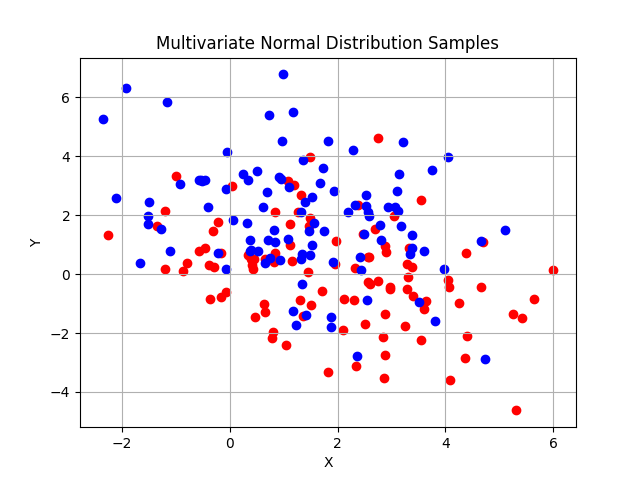
\includegraphics[width=0.8\textwidth]{4(1)散点图.png}

(2)fisher|伪逆|梯度下降法求解权值向量的结果如下图:

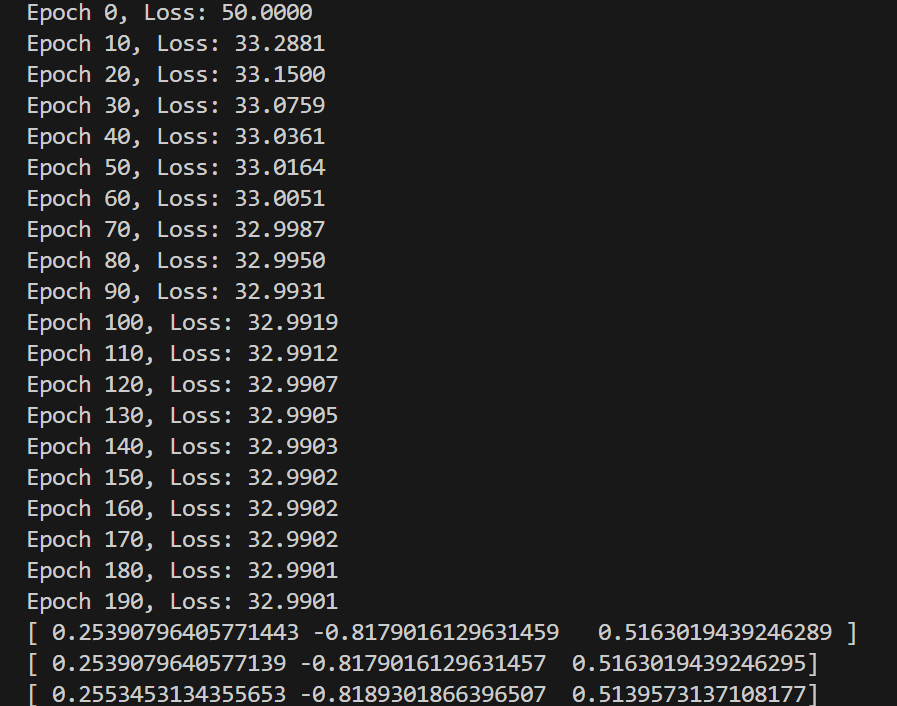
\includegraphics[width=0.8\textwidth]{梯度下降过程及最终向量.png}\\
包括梯度下降过程中的损失函数loss值的变化(这里采用均方误差作为损失函数)\\
(3)最终图像如下:\\
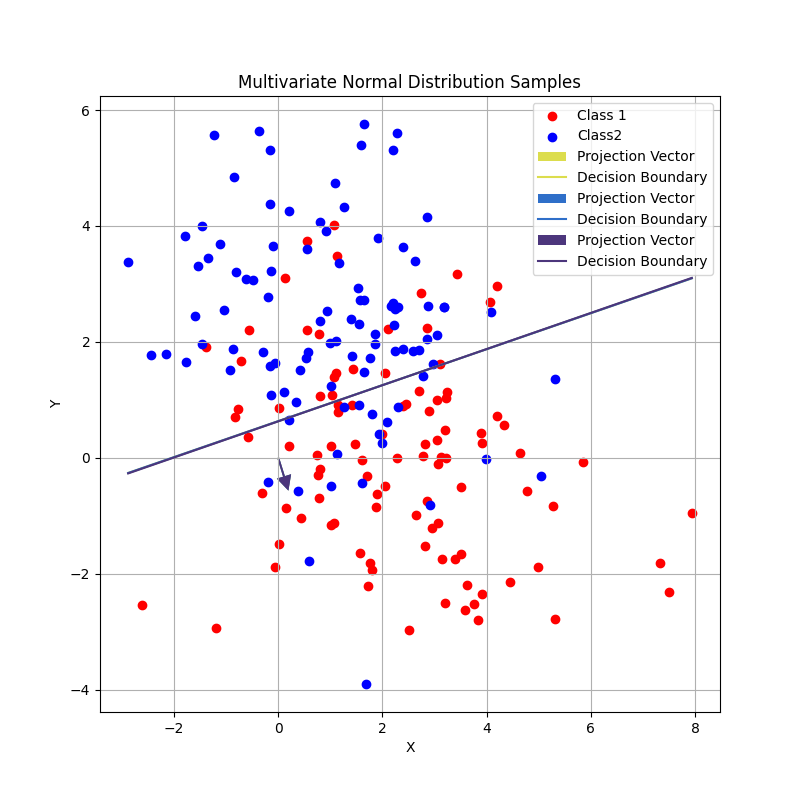
\includegraphics[width=0.8\textwidth]{T4.png}\\
由图(2)(3)可知:\\
(i)Fisher判别方法和伪逆矩阵法得到的权值向量$w$和分类超平面几乎完全相同,权值向量归一化后仅在小数点后15位后有差异;\\
(ii)采用学习率阶梯衰减的方法,梯度下降法最终也能很好地拟合曲线,得到的权值向量和分类超平面几乎重合.

python代码如下:
\begin{verbatim}
    import numpy as np
    import matplotlib.pyplot as plt
    #常量定义
    mean1=[2,0]
    cov=[[3,-1],[-1,3]]
    num=100
    mean2=[1,2]
    #生成样本
    sample1=np.random.multivariate_normal(mean1,cov,num)
    sample2=np.random.multivariate_normal(mean2,cov,num)
    #添加偏置项
    sample1_new=np.hstack([sample1,np.ones((num,1))])
    sample2_new=np.hstack([sample2,np.ones((num,1))])
    #合并样本方便使用
    X = np.vstack([sample1_new, sample2_new])
    y=np.array([1 if i<num else -1 for i in range(2*num)])#添加真实标签
    
    #1.Fisher线性判别法
    m1=np.mean(sample1, axis=0)
    m2=np.mean(sample2, axis=0)
    S_W = np.zeros((2, 2))
    for i in range(len(sample1)):
        S_W += np.outer(sample1[i] - m1, sample1[i] - m1)
    for i in range(len(sample2)):
        S_W += np.outer(sample2[i] - m2, sample2[i] - m2)
    # 投影向量 w_1
    w_0=np.linalg.inv(S_W).dot(m1-m2)
    origin=-w_0.dot((m1+m2)/2)
    w_1=np.append(w_0,origin)#添加偏置项
    
    #2.伪逆方法
    X_pinv = np.linalg.pinv(X)
    w_2= X_pinv.dot(y)
    
    #3.梯度下降法
    w_3 = np.zeros(3)
    eta = 0.0005
    decay_rate=0.9
    decay_steps=40
    T=200
    for t in range(T):
        y_pred=X.dot(w_3)
        #计算梯度
        grad=-X.T.dot(y-y_pred)#X.T是转置矩阵
        #更新学习率eta
        if t % decay_steps == 0:
            eta = eta * decay_rate
        w_3=w_3-eta*grad
        # 每隔10次迭代输出一次损失函数值
        if t % 10 == 0:
            loss = (1/2*num)*np.mean((y_pred - y) ** 2)
            print(f"Epoch {t}, Loss: {loss:.4f}")
    
    #绘制样本点
    plt.figure(figsize=(8, 8))
    plt.scatter(sample1[:,0],sample1[:,1],c='r',marker='o',label='Class 1')
    plt.scatter(sample2[:,0],sample2[:,1],c='b',marker='o',label='Class2')
    plt.title('Multivariate Normal Distribution Samples')
    
    for w in (w_1,w_2,w_3):
        # 归一化向量w
        norm = np.linalg.norm(w)#计算模长
        w_normalized = w / norm
        np.set_printoptions(precision=20)#控制打印精度
        print(w_normalized)
        random_color = np.random.rand(3,)  # 生成一个随机颜色
        #从原点出发绘制投影向量
        plt.quiver(0, 0, w[0], w[1], angles='uv',width=0.003, headwidth=8, headlength=8, headaxislength=8, color=random_color, label='Projection Vector')
        # 计算决策面(线性判别函数)
        x_vals = np.linspace(min(X[:, 0]), max(X[:, 0]), 100)
        y_vals = (-w[0] / w[1])* x_vals - (w[2] / w[1])
        plt.plot(x_vals, y_vals, color=random_color, label='Decision Boundary')
    
    plt.legend()#设置图例
    plt.xlabel('X')
    plt.ylabel('Y')
    plt.grid(True)
    plt.show()
\end{verbatim}



\end{document}
